\section{Materiales y métodos}

En esta sección, describiremos la metodología utilizada en el estudio de la Disgrafia,
junto con los materiales empleados. La metodología se dividió en varias etapas, las
cuales se detallarán a lo largo de esta sección y se pueden observar en la imagen \ref{fig:workflow}.

\begin{figure}[h!]
	\centering
	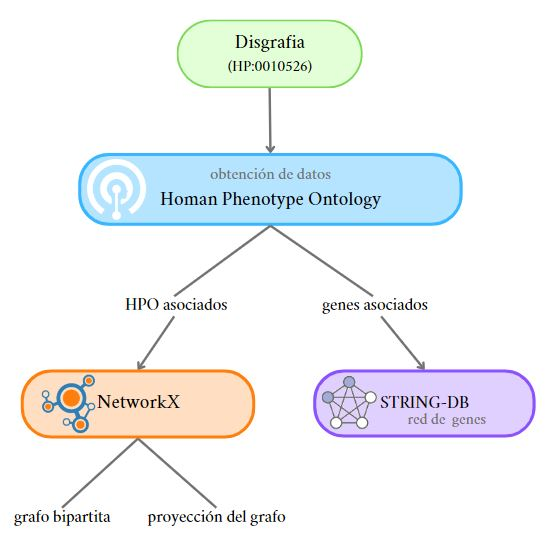
\includegraphics[width=0.7\textwidth]{figures/workflow.JPG}
	\caption{Flujo de trabajo}
	\label{fig:workflow}
\end{figure}

\subsection{Datos biológicos}

Lo primero que se realizó fue descargar los dataset necesarios para hacer el estudio. Se usaron dos base de datos: Human Phenotype Ontology (HPO) \cite{HPO2021} y STRING-DB \cite{String2021}.

\begin{enumerate}
	\item Se buscó el fenotipo Disgrafía en la HPO, conociendo que su identificador es HP:0010526. De esta base de datos, obtuvimos dos archivos tabulados; uno contiene los genes asociados y el otro contiene términos HPO asociados a la Disgrafía.
	\item La base de datos STRING se usó para descargar la red de interacción de proteínas humanas
\end{enumerate}


A continuación, se van a describir los distintos conjuntos de datos mencionados anteriormente.

\begin{itemize}
	\item \textbf{HPO asociados}
\end{itemize}

Uno de los archivos enumera para cada gen las clases HPO más específicas. Las primeras cinco filas se pueden visualizar en la tabla \ref{tabla:geneshpo}.

\renewcommand{\arraystretch}{1.5} % add more vertical space between cells in the table

\begin{table}[h!]
	\centering
	\caption{Cabecera del archivo de HPO asociados}
	\label{tabla:geneshpo}
	\resizebox{1.1\textwidth}{!}{
		\begin{tabular}{|c|c|c|c|c|c|c|}
			\hline
			Gene id (ncbi) & Gene symbol & HPO id & HPO name & frequency & Disease id \\
			\hline
			10 & NAT2 & HP:0000007 & Autosomal recessive inheritance & - & OMIM:243400 \\
			10 & NAT2 & HP:0001939 & Abnormality of metabolism/homeostasis & - & OMIM:243400 \\
			16 & AARS1 & HP:0002460 & Distal muscle weakness & 15/15 & OMIM:613287 \\
			16 & AARS1 & HP:0002451 & Limb dystonia & 3/3 & OMIM:616339 \\
			16 & AARS1 & HP:0008619 & Bilateral sensorineural hearing impairment & HP:0040283 & ORPHA:33364 \\
			\hline
		\end{tabular}
	}
\end{table}

La tabla \ref{tabla:geneshpo} proporciona el identificador de gen NCBI, el símbolo del gen, el identificador HPO y el nombre del término. Si está disponible, se muestra la frecuencia. Para este campo, hay tres opciones:

\begin{enumerate}
	\item Un identificador de término dentro de la sub-ontología de la HPO que esté relacionado con la frecuencia del fenotipo en cuestión
	\item Un recuento de pacientes afectados dentro de un individuo. "7/13" indicaría que 7 de los 13 pacientes con la enfermedad especificada tienen la anormalidad fenotípica mencionada por el término de la HPO en cuestión. Por ejemplo, la mutación en el gen AARS1 causa \textit{leucoencefalopatía}. La frecuencia del término HPO Ataxia sensorial esta anotada como 1 de 2 debido a la información en Sundal C, et al. \cite{Sundal2019}. 
	\item Un valor porcentual. Nuevamente, esto se refiere al porcentaje de pacientes que tienen la anormalidad fenotípica mencionada por el término de la HPO.
\end{enumerate}

La última columna muestra anotaciones realizadas por el equipo HPO (utilizando identificadores de enfermedades de OMIM), así como anotaciones proporcionadas por el equipo de Orphanet \cite{Orphanet2008} (utilizando identificadores de enfermedades de ORPHA).

El archivo se introdujo en Python como un data frame utilizando la librería Pandas \cite{pandasPython}. A través de operaciones lógicas aplicadas al data frame, se intentó inferir la existencia de algún gen que estuviera exclusivamente relacionado con la Disgrafía, sin tener asociación con otro término HPO.

\begin{itemize}
	\item \textbf{Genes asociados}
	\label{section:genesAsociados}
\end{itemize}

El segundo archivo consiste en un listado de genes asociados a la disgrafía. En la tabla \ref{tabla:genesAsociados}, se presenta la cabecera del archivo, donde también se visualizan tres columnas: la primera contiene el identificador de Entrez de los genes, la segunda el símbolo de los genes y la tercera el identificador de las enfermedades. Al igual que en el archivo anterior, el identificador de las enfermedades puede provenir de dos fuentes, OMIM o Orphanet.

\begin{table}[h]
	\centering
	\caption{Cabecera del archivo de genes asociados}
	\label{tabla:genesAsociados}    
	\resizebox{\textwidth}{!}{
		\begin{tabular}{|c|c|c|}
			\hline
			Gene id (entrez) & Gene symbol & DISEASE\_IDS \\
			\hline
			10347 & ABCA7 & ORPHA:1020,OMIM:608907 \\
			351 & APP & OMIM:605714,ORPHA:100006,ORPHA:1020,ORPHA:3247... \\
			9031 & BAZ1B & ORPHA:904 \\
			9275 & BCL7B & ORPHA:904 \\
			657 & BMPR1A & OMIM:174900,ORPHA:329971,OMIM:610069,ORPHA:157... \\
			\hline
		\end{tabular}
	}
\end{table}

\begin{itemize}
	\item \textbf{Red proteínas}
\end{itemize}

Este archivo contiene una red de interacciones entre proteínas humanas, presentes en la base de datos STRING, junto con una puntuación de los enlaces entre las proteínas. La cabecera de este archivo se puede visualizar en la tabla \ref{tabla:redProteinas}.

%\newcolumntype{C}{>{\centering\arraybackslash} p{4.5cm} }

\begin{table}[h]
	\centering
	\caption{Datos de la red de proteínas con puntuaciones combinadas.}
	\label{tabla:redProteinas} 
	\begin{tabular}{|c|c|c|}
		\hline
		\textbf{Proteína 1} & \textbf{Proteína 2} & \textbf{Puntuación Combinada} \\
		\hline
		9606.ENSP00000000233 & 9606.ENSP00000356607 & 173 \\
		9606.ENSP00000000233 & 9606.ENSP00000427567 & 154 \\
		9606.ENSP00000000233 & 9606.ENSP00000253413 & 151 \\
		9606.ENSP00000000233 & 9606.ENSP00000493357 & 471 \\
		\hline
	\end{tabular}
\end{table}

Cada fila contiene el StringID de las dos proteínas que interactúan, junto con el \textit{combined score}. Esta puntuación se calcula al combinar las probabilidades de diferentes canales de evidencia y se corrige por la probabilidad de observar una interacción al azar.

Este archivo es demasiado grande para subirlo al repositorio, por lo que se ha filtrado por el \textit{combined score} utilizando expresiones regulares:

\begin{verbatim}
	awk -F" " '$3 > 800 {print $0}'
	9606.protein.links.v12.0.txt > proteinas_filtrado.txt
\end{verbatim}

De esta forma, nos quedamos con aquellas interacciones que tengan una puntuación mayor a 800.

\subsection{Grafo bipartito}

Al no encontrarse ningún gen que afecte solo a Disgrafía, se buscó aquellos términos HPO relacionados [...]

En un grafo bipartito, los vértices se organizan en dos conjuntos distintos, de modo que cada arista conecta un vértice de un conjunto con otro del segundo conjunto. En términos más simples, no existen aristas que conecten vértices dentro del mismo conjunto \cite{BiRank2017}. En nuestro contexto, los conjuntos de vértices representan genes y términos HPO. De esta manera, obtenemos un grafo bipartito que conecta distintos términos HPO al nuestro, a través de genes. 

Para llevar a cabo esta representación y conexión entre genes y términos HPO, hemos utilizado la librería de Python NetworkX \cite{BookNetworkX}. Usando las segunda y tercera columna de la tabla \ref{tabla:geneshpo}, es decir los símbolos de los genes y los identificadores de los términos HPO, se creó este grafo bipartito. [...]

De este grafo nos interesaba ver aquellos término HPO que se encuentran estrechamente relacionados con la Disgrafía, por lo que lo siguiente que hicimos fue hacer un subgrafo que con los nodos que se encuentre a dos pasos del término HPO Disgrafía y hacer una proyección de los términos HPO de ese subgrafo. De esta forma obtuvimos aquellos HPO que están relacionados con al Disgrafía a través de un gen. [...].

\subsection{Red de genes}

A continuación, se procedió a realizar un estudio de los genes relacionados con la disgrafía (usando el archivo descrito en \ref{section:genesAsociados}). Lo primero fue obtener la red de genes utilizando la API de String-DB \cite{String2021}, haciendo uso de la biblioteca \textit{strindb} para Python. Entre las funciones clave de esta biblioteca se encuentra get\_network, la cual requiere como parámetros la lista de nuestros genes y el identificador de la especie \textit{Homo sapiens} (9606). Adicionalmente, se ha impuesto un score de 500, esta es una puntuación de corte para los bordes de la red, corresponde a la probabilidad de pertenecer a la misma vía funcional, lo que se traduce en que salgan más o menos genes en nuestra red.

La función devuelve la red de genes, donde se encuentran representados los genes y las relaciones entre ellos, la cual guardamos en un archivo .tsv.


\subsection{Propagación de la red}

Una vez que tenemos la red con los genes asociados, llevamos a cabo una propagación de la red con el objetivo de ampliar su tamaño y buscar otros genes relacionados con la Disgrafía. Este enfoque nos permite potencialmente descubrir otros genes implicados en la Disgrafía.

Para llevar a cabo este proceso, existen diferentes algoritmos, entre los cuales hemos seleccionado Diamond \cite{Diamond2015}.

Este algoritmo toma como parámetros nuestra red de genes, la red de interacciones de proteínas (filtrada), el número de genes que queremos que tenga el grafo final, y el nombre del archivo donde se va a guardar la red ampliada.

\begin{verbatim}
	python DIAMOnD.py proteinas_filtrado.txt grafo_51_genes.txt 200
	propaged_genes.txt
\end{verbatim}

\subsection{Detección de comunidades}

Para estudiar el grafo ampliado y la relación de los nuevos genes añadidos con el HPO de interés, se ha llevado a cabo un análisis de comunidades.

La detección de comunidades consiste en fragmentar el grafo en conjuntos de nodos, denominados "comunidades", teniendo en cuenta la topología de la red. En resumen, puede conceptualizarse como un proceso de agrupamiento (clustering) aplicado a grafos. Aunque no hay una definición única de comunidad aceptada por la comunidad científica, generalmente se considera que una comunidad es de calidad cuando muestra más conexiones internas que externas. En otras palabras, los nodos dentro de la comunidad están más densamente conectados entre sí en comparación con los nodos fuera de la comunidad en el grafo \cite{PanizoLledot}.

Para hacer la detecciónn de comunidades del grafo se ha usado uno de los algortimos proporcionados por el paquete NetworkX,\textit{ greedy\_modularity\_communities}. Este algoritmo utiliza la maximización de modularidad avariciosa de Clauset-Newman-Moore \cite{Clauset2004} para encontrar la partición de comunidades con la mayor modularidad.


\subsection{Enriquecimiento funcional}

El análisis funcional de genes implica registrar y analizar estadísticamente listas de genes con el objetivo de identificar anotaciones funcionales en relación con los genes analizados. El propósito principal es determinar si existe una asociación significativa entre los genes y las funciones específicas que desempeñan en procesos biológicos, rutas metabólicas u otras categorías funcionales. 

El enriquecimiento funcional se ha llevado a cabo utilizando el paquete String de Python, específicamente la función \textit{get\_enrichment}. Este análisis se ha realizado en varias ocasiones: una vez para el grafo ampliado y otra para cada una de las comunidades detectadas en la sección anterior.